% !TeX spellcheck = en_US
%
%
% v 2.3  Feb 2019   Volker RW Schaa
%		# changes in the collaboration therefore updated file "jacow-collaboration.tex"
%		# all References with DOIs have their period/full stop before the DOI (after pp. or year)
%		# in the author/affiliation block all ZIP codes in square brackets removed as it was not
%         understood as optional parameter and ZIP codes had bin put in brackets
%       # References to the current IPAC are changed to "IPAC'19, Melbourne, Australia"
%       # font for "url" style changed to "newtxtt" as it is easier to distinguish "O" and "0"
%
\documentclass[letter,
               %boxit,        % check whether paper is inside correct margins
               %titlepage,    % separate title page
               %refpage       % separate references
               biblatex,     % biblatex is used
               keeplastbox,   % flushend option: not to un-indent last line in References
               %nospread,     % flushend option: do not fill with whitespace to balance columns
               %hyphens,      % allow \url to hyphenate at "-" (hyphens)
               %xetex,        % use XeLaTeX to process the file
               %luatex,       % use LuaLaTeX to process the file
               ]{jacow}
%
% ONLY FOR \footnote in table/tabular
%
\usepackage{pdfpages,multirow,ragged2e} %
%
% CHANGE SEQUENCE OF GRAPHICS EXTENSION TO BE EMBEDDED
% ----------------------------------------------------
% test for XeTeX where the sequence is by default eps-> pdf, jpg, png, pdf, ...
%    and the JACoW template provides JACpic2v3.eps and JACpic2v3.jpg which
%    might generates errors, therefore PNG and JPG first
%
\makeatletter%
	\ifboolexpr{bool{xetex}}
	 {\renewcommand{\Gin@extensions}{.pdf,%
	                    .png,.jpg,.bmp,.pict,.tif,.psd,.mac,.sga,.tga,.gif,%
	                    .eps,.ps,%
	                    }}{}
\makeatother

% CHECK FOR XeTeX/LuaTeX BEFORE DEFINING AN INPUT ENCODING
% --------------------------------------------------------
%   utf8  is default for XeTeX/LuaTeX
%   utf8  in LaTeX only realises a small portion of codes
%
\ifboolexpr{bool{xetex} or bool{luatex}} % test for XeTeX/LuaTeX
 {}                                      % input encoding is utf8 by default
 {\usepackage[utf8]{inputenc}}           % switch to utf8

\usepackage[USenglish]{babel}

%%   Lengths for the spaces in the title
%%   \setlength\titleblockstartskip{..}  %before title, default 3pt
%%   \setlength\titleblockmiddleskip{..} %between title + author, default 1em
%%   \setlength\titleblockendskip{..}    %afterauthor, default 1em

%----------------------------------------------------------

%\usepackage{subfig}
%\usepackage[final]{pdfpages}
%\usepackage{multirow}
%\usepackage{ragged2e}
%\usepackage{fixmath}
%\usepackage{alltt}
%\usepackage{xspace}
%\usepackage[strings]{underscore}    % to use "_" in text

%
% if BibLaTeX is used
%

\addbibresource{converter.bib}
\graphicspath{{figures/}}

\newcommand{\bmad}{\textit{Bmad}}
\newcommand{\xx}{\mathbf{\hat{x}}}
\newcommand{\yy}{\mathbf{\hat{y}}}
\newcommand{\zz}{\mathbf{\hat{z}}}
\newcommand{\rr}{\mathbf{\hat{r}}}
\newcommand{\rrr}{\mathbf{r}}
\newcommand{\dxds}{\frac{dx}{ds}}
\newcommand{\dyds}{\frac{dy}{ds}}

%----------------------------------------------------

%----------------------------------------------------
\begin{document}

\title{Simulating a Positron Converter in Bmad}

\author{Authors, Cornell University, Ithaca, NY, 14850, USA}

\maketitle

%----------------------------------------------------
\begin{abstract}
Abstract
\end{abstract}

%----------------------------------------------------
\section{Introduction}

%TODO: add references

Electron-positron accelerators require a source of positrons.
The standard method of obtaining positrons for use in an accelerator is through the use of a positron converter.
This is typically a slab of heavy metal, such as tungsten, located in a linear branch of the accelerator.
The converter is bombarded with electrons with energies of order $\sim 100$ MeV.
The electrons emit photons via Bremsstrahlung, which in turn decay to $e^+ e^-$ pairs:
\begin{align*}
e^- + Z \rightarrow e^- + Z + \gamma \rightarrow e^- + Z + e^- + e^+.
\end{align*}
The electrons are then quickly filtered off with a %TODO: what kind of?
magnet, effectively "convertering" a beam of incoming electrons into a beam of outgoing positrons.

There is some discussion in the literature regarding the Bremsstrahlung energy spectrum in various materials, %TODO: cite
as well as the energy spectra of the $e^+ e^-$ secondaries. %TODO: cite
However, there is no closed form, analytical solution that describes the kinematics of the emitted $e^+$ in terms of the kinematics of the incoming $e^-$ and the physical properties of the converter.

Previous attempts have also been made at developing numerical models of a positron converter. %TODO: cite Fromowitz
However, these results have been highly specialized, and have been completely standalone solutions. %TODO: elaborate
There has also been a recent demand for modelling the transfer of spin from the incoming beam of electrons to the outgoing beam of positrons. %TODO: add citation

In response, the authors have developed a positron converter model for use with the \bmad{} accelerator toolkit.
Our model is designed to be as flexible as possible, accomadating any converter material and thickness.
The model can even be extended to support other kinds of incoming and outgoing particles, and is not limited to taking electrons in and sending positrons out.
The model is also fast to use within \bmad{}, with the expensive physics calculations performed only once as the converter model is being developed. %TODO: reword this

This converter model enables \bmad{} users to optimize the design of lattices that contain positron converters.
This was not previously possible, as there was no way to simulate the effects of a converter within \bmad{}. %TODO: elaborate or fold into the previous paragraph


%----------------------------------------------------
\section{The Converter Model}

The physical processes that occur in the positron converter to produce the Bremsstrahlung photons and subsequent positrons are governed by quantum electrodynamics. %TODO: maybe add a reference?
The details of these interactions are not critical when only the aggregate behavior of the converter is of interest.
Therefore, the converter's behavior is modelled with a probability distribution, which describes the overall distribution of the produced positrons in terms of the target and incoming electron's properties. %TODO: reword

\subsection{Coordinate System}

Consider an electron incident on the upstream face of a positron converter of thickness $T$, with momentum $p_- c$ perpendicular to the face of the converter as depicted in \ref{fig:coords1}.
Positrons produced in the converter emerge from the downstream face with some radial displacement $r$ and at an angle $\theta$ relative to the horizontal, as depicted in \ref{fig:coords2}.
The direction of the radial displacement defines for each outgoing positron an $\xx$ and $\yy$ axis, with $\xx$ taken in the same direction as $\rrr$, and $\yy$ taken so that $(\xx, \yy, \mathbf{s})$ is a right-handed orthogonal coordinate system.

By symmetry, $\theta$ must be uniformly distributed from 0 to $2\pi$.
Therefore, the kinematic properties of the produced positrons which must be modelled are its radial displacement and outgoing momentum.
The outgoing momentum $\mathbf{p}_+ c$ is described in terms of its magnitude, $p_+ c$, and its slopes along the $\xx$ and $\yy$ directions:
\begin{align}
\frac{dx}{ds} & = \frac{p_x}{p_s} \\
\frac{dy}{ds} & = \frac{p_y}{p_s}.
\end{align}


%TODO: match figure font to document font
\begin{figure}
\centering
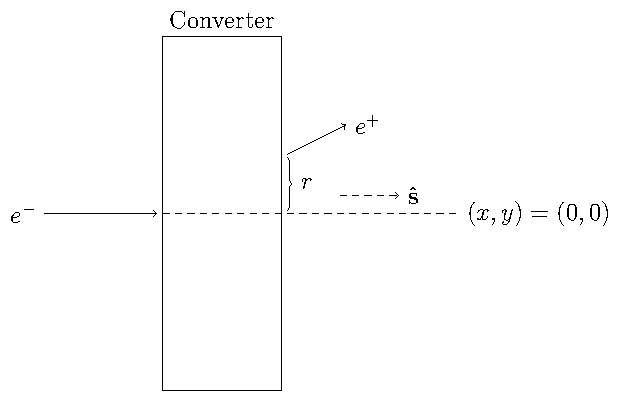
\includegraphics[width=0.45\textwidth]{coords1.pdf}
\caption{Positron converter coordinate system (side view).}
\label{fig:coords1}
\end{figure}

%TODO: make the bounding box on this figure smaller
\begin{figure}
\centering
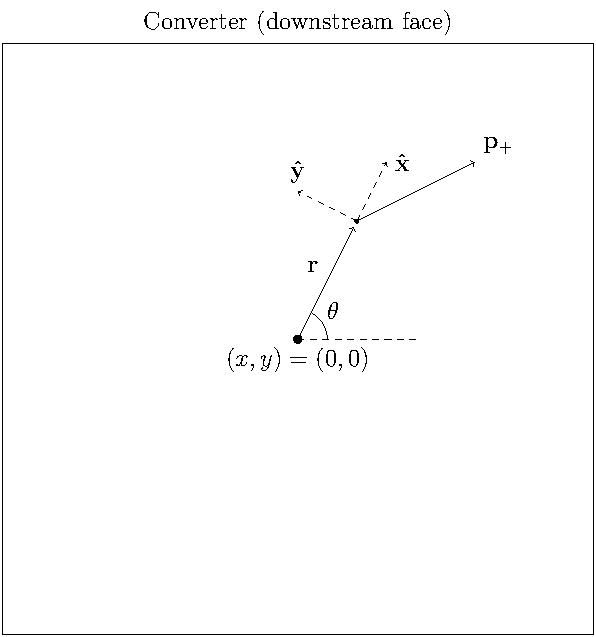
\includegraphics[width=0.4\textwidth]{coords2.pdf}
\caption{Positron converter coordinate system (view of the downstream face).}
\label{fig:coords2}
\end{figure}

\subsection{Probability Distributions}

Positrons produced in the converter are described by the distribution
\begin{align}
P \left( p_+ c, r, \dxds, \dyds \right)
\end{align}
which indicates the probability that an outgoing positron will have a given momentum and radial displacement.
$P$ is normalized to account for the efficiency of positron production:
\begin{align}
\int P \left( p_+ c, r, \dxds, \dyds \right) \, d(p_+ c) \, dr \, d \! \left( \dxds \right) d \! \left( \dyds \right) & = \frac{N_+}{N_-},
\end{align}
where $N_+$ is the total number of positrons produced, and $N_-$ is the number of electrons incident upon the converter.
To make the problem easier to grapple with, $P$ is decomposed into two subdistributions,
\begin{align}
P \left( p_+ c, r, \dxds, \dyds \right) & = P_1 \left( p_+ c, r \right) P_2 \left( \dxds, \dyds ; p_+ c, r \right)
\end{align}
which are normalized to $N_+/N_-$ and $1$ respectively.
Note that $P_2$ depends on $p_+ c$ and $r$, so that the shape of $P_2$ may vary with $p_+ c$ and $r$.

Using Geant\cite{geant}, a large number of electrons incident upon the converter are simulated, and the produced positrons and their kinematics are recorded.
The produced positrons are binned into a two-dimensional histogram by their $p_+ c$ and $r$ values.
This histogram gives an approximation of $P_1$.
For $P_2$, fits are performed to $\dxds$ and $\dyds$ for the positrons in each $(p_+c, r)$ bin.
These fits yeild $P_2 \left( \dxds, \dyds ; p_+ c, r \right)$.
Examples of the $P_1$ and $P_2$ distributions obtained from the Geant simulation are shown in Figures \ref{fig:p1} and \ref{fig:p2} respectively.

\begin{figure}
\centering
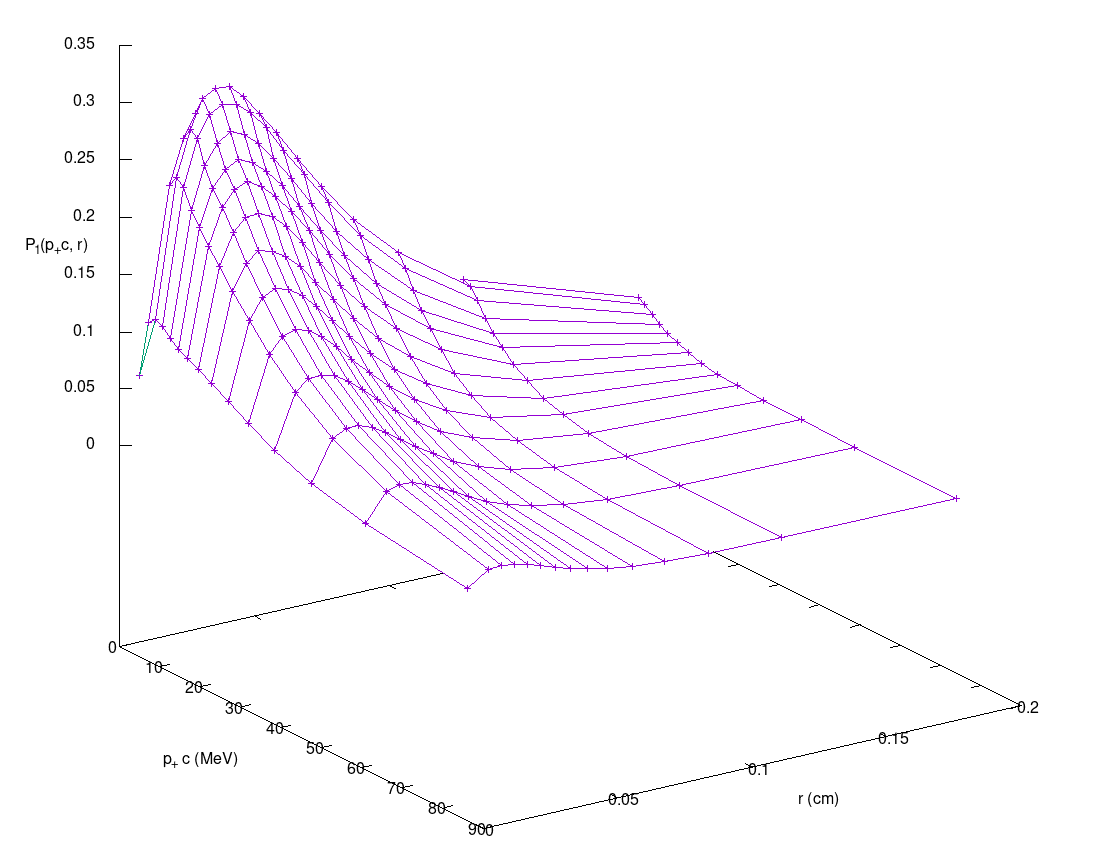
\includegraphics[width=0.45\textwidth]{p1}
\caption{$P_1(p_+ c, r)$ for incoming electrons with $p_- c = 300$ MeV and a tungsten target of thickness $T = 6.35$ mm.}
\label{fig:p1}
\end{figure}

\begin{figure}
\centering
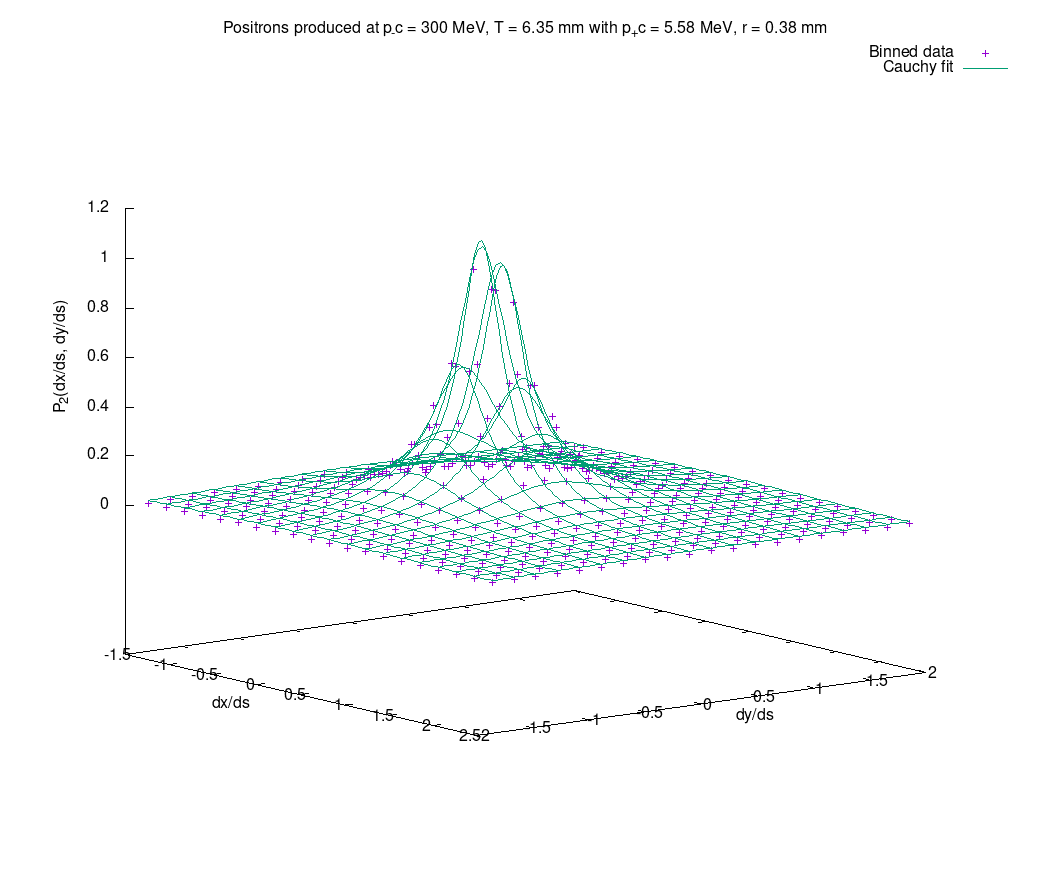
\includegraphics[width=0.45\textwidth]{p2}
\caption{$P_2 \left( \dxds, \dyds ; p_+ c, r \right)$ for incoming electrons with $p_- c = 300$ MeV and a tungsten target of thickness $T = 6.35$ mm,
and outgoing positrons with $p_+ c = 5.58$ MeV and $r = 0.38$ mm.
The purple points indicate data obtained directly from the Geant simulation, while the green curve shows the fit to the data.
}
\label{fig:p2}
\end{figure}

%\begin{itemize}
%\item
%Paraphrase and condense what is written in the documentation
%
%\end{itemize}


\section{Spin Tracking}

Polarization transfer from the incoming electrons to the outgoing positrons has also been modelled.
Any incoming polarization $\mathbf{S}_-$ may be specified, and histograms describing $S_x$, $S_y$, and $S_z$ of the produced positrons as functions of $p_+ c$ and $r$ are produced.
The authors have found that only the longitudinal polarization of the incoming electrons is ever transferred to the produced positrons; the produced positrons always have $S_x$ and $S_y$ essentially zero regardless of the incoming electron polarization.
As an example, Figure \ref{fig:sz} illustrates $S_z$ as a function of $p_+ c$ and $r$ for incoming electron with momentum $p_- c = 300$ MeV.

\begin{figure}
\centering
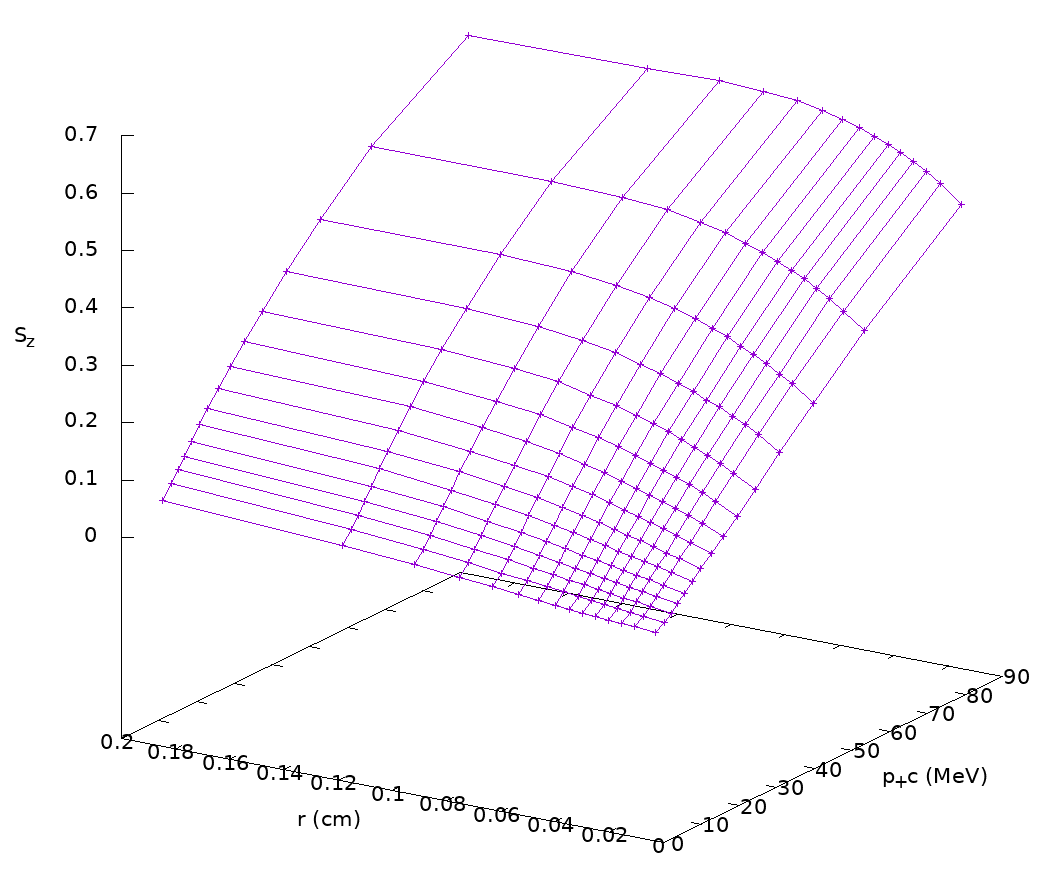
\includegraphics[width=0.45\textwidth]{sz}
\caption{Positron $S_z$ as a function of $p_+ c$ and $r$ for incoming electrons with $p_- c = 300$ MeV and a tungsten target of thickness $T = 6.35$ mm.}
\label{fig:sz}
\end{figure}

\begin{itemize}
\item
Discuss 2016 PRL

\item
Compare our simulation output to their experimental results

\end{itemize}


%\begin{itemize}
%\item
%Give general description of how spin is recorded from the simulation
%
%\item
%Discuss results/planned experimental verification?
%
%\end{itemize}


%----------------------------------------------------
\section{The Bmad Converter Element}

\begin{itemize}
\item
Describe how simulation output is read into Bmad

\item
Discuss Bmad's scheme for generating positrons from simulation output

\item
Compare Bmad/Geant distributiions?

\end{itemize}


%----------------------------------------------------
\section{Applications}

\begin{itemize}
\item
CESR Linac lattice

\item
Optimizations could include
\begin{itemize}
\item
Tuning quad/solenoid strengths

\item
Tuning element positions

\end{itemize}

\item
Discuss increase in yield due to optimizations that were made possible by the converter element?

\end{itemize}


%----------------------------------------------------
\section{Conclusion}

%--------------------------------------------------------------------------------------
\section{Acknowledgments}

Many thanks to Vardan Khachatryan for getting us up and running with Geant.
% and any other help relevant to obtaining linac lattice,
% funding etc

%--------------------------------------------------------------------------------------

\printbibliography

\clearpage

\end{document}

